\subsection{Hyperblock}

\begin{definition}[Hyperblock]
Hyperblock是一个谓词化的基本块的集合,这个集合只有一个入口,但是可以有多个出口。
\end{definition}

哪些基本块被包含在Hyperblock中,哪些不被包含在Hyperblock中,这个的选择比较自由,可以根据需要选择,比如说把不经常被执行的基本块,或者太过长的基本块排除在外,而把经常执行又短小精悍的基本块包含在内。
自由选择的基本块不一定满足Hyperblock的定义,比如\fref{fig:taildup}以及\fref{fig:looppeeling}的(a),这时候就需要对控制流图进行一定的处理,这样才能使选择的基本块能够构成一个Hyperblock。

对不满足定义的基本块的集合处理的一种变换是\textbf{尾复制(Tail Duplication)},另一种是\textbf{循环剥离(loop peeling)}。尾复制过程如\fref{fig:taildup}所示,图中(a)是分支选择的结果,(b)是尾复制以后的结果,(c)是if-conversion之后的结果。
\begin{figure}
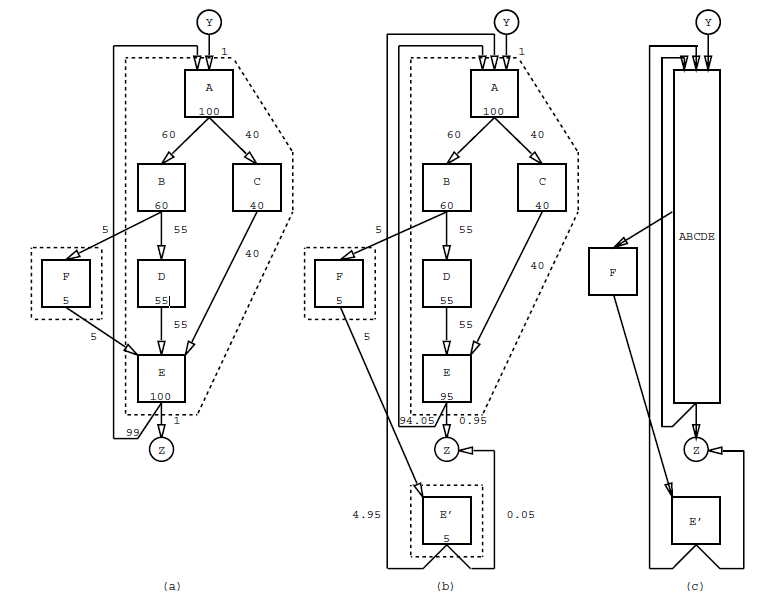
\includegraphics[width=\linewidth]{mechanism/hyperblock-td}
\caption{\label{fig:taildup} 尾复制}
\end{figure}

循环剥离的过程如\fref{fig:looppeeling}所示,图中(a)是分支选择的结果,(b)是循环剥离以后的结果。
\begin{figure}
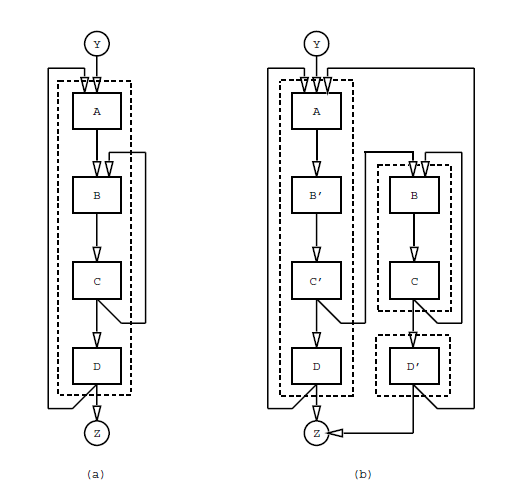
\includegraphics[width=\linewidth]{mechanism/hyperblock-lp}
\caption{\label{fig:looppeeling} 循环剥离}
\end{figure}
